%! Author = jakobnieder
%! Date = 07.02.24


\section{Color term background}
\label{sec:Color_term_background}

\textcite{berlinBasic1969} collected color naming data on 320 chromatic and nine non-chromatic Munsell chips (\textcite{lennebergLanguage1956}; see Figure \ref{fig:munsell-chips}) from speakers of 20 languages in the Bay Area. Most of these speakers were bilingual. In a follow-up project, the ``World Color Survey" (WCS), linguists and anthropologists from around the world studied color naming patterns in 110 unwritten languages, many of them in small societies (Fig \ref{fig:wcs-locations}).

\begin{figure}[htbp]
\centering
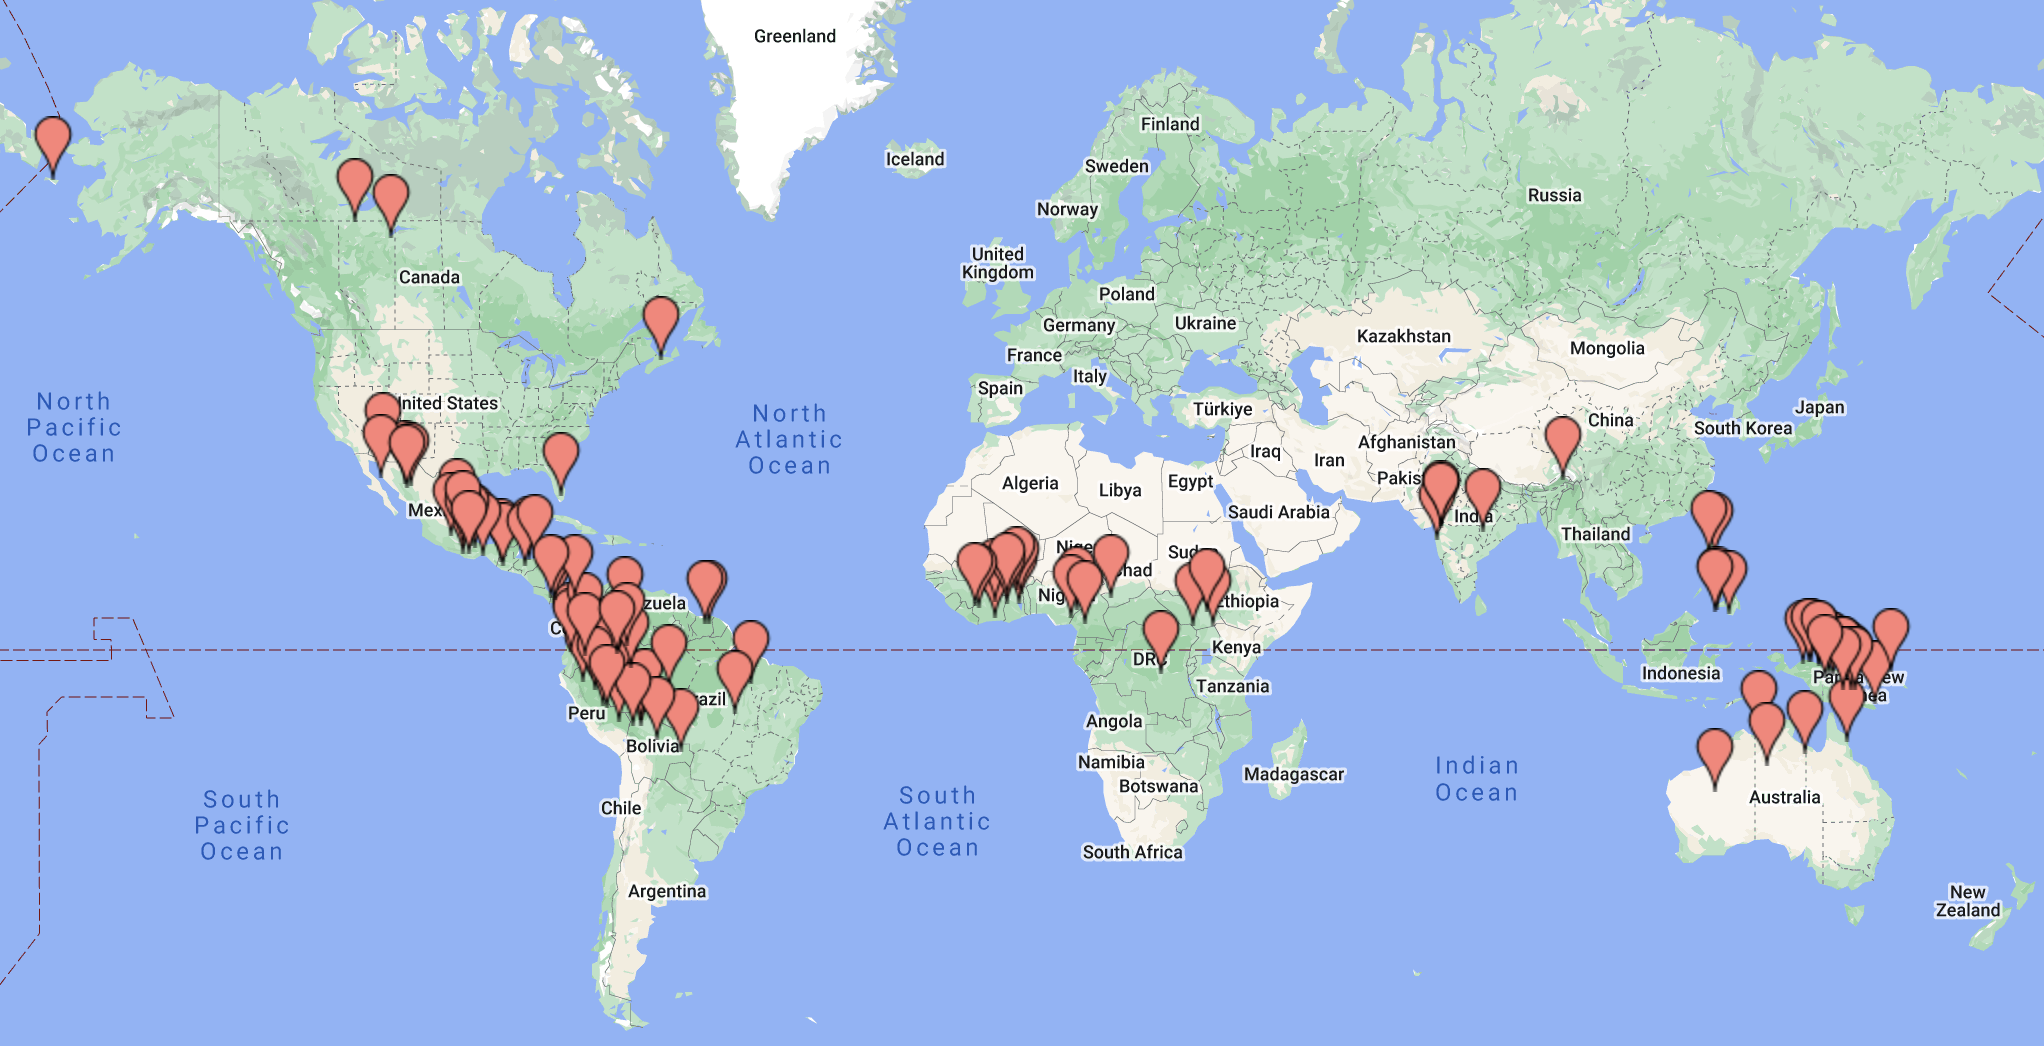
\includegraphics[width=\linewidth]{images/wcs-locations.png}
\decoRule
\caption[WCS Locations]{World map with information on the location of the 110 languages examined in the WCS.}
\label{fig:wcs-locations}
\end{figure}

Here, they used 330 Munsell chips, including 329 Munsell chips from the earlier study, plus one white chip. Their method included two stages. First, in a free naming task, participants named each chip in a fixed randomized order. In a second task (``focus task"), participants were asked to point to the color chip that best represents each unique color term used in the first task. This study concluded that having ``basic colors" -- a small set of commonly used color terms -- is universal. 

The systems of color terms themselves, however, varied greatly across languages. Nevertheless, they showed that languages with similar numbers of BCT tend to have similar mappings of terms to colors. Based on this, Berlin and Kay suggested that color terms systems develop from the simplest two color terms systems to more complex color systems with up to eleven color terms (\textit{black, white, red, yellow, green, blue, brown, orange, pink, purple, and gray})\parencite{berlinBasic1969,kayWorld2016}. According to this hypothesis, languages with similar numbers of terms have similar color maps because they went through the same constrained historical development trajectory. They received support by an approach by \textcite{lindseyUniversality2006} using k-means clustering, taking the naming pattern of each WCS participants as input. This analysis revealed successively forking categories from two to ten. The step wise results resembled with exceptions very well the actual categories present in the examined WCS languages and english. In addition, they identified regions of low concordance dividing roughly warm and cold colors across participants in color space. Both findings indicate consistent tendencies across languages dependent on the number of color terms.
\parencite{lindseyUniversality2006}

Across all WCS languages, \textcite{lindsey2009World} were able to categorize individual differences into six motives, reflecting the use of different subsets of BCT. The presence of two motives was replicated for English \parencite{lindseyColor2014}.

\begin{figure}[htbp]
\centering
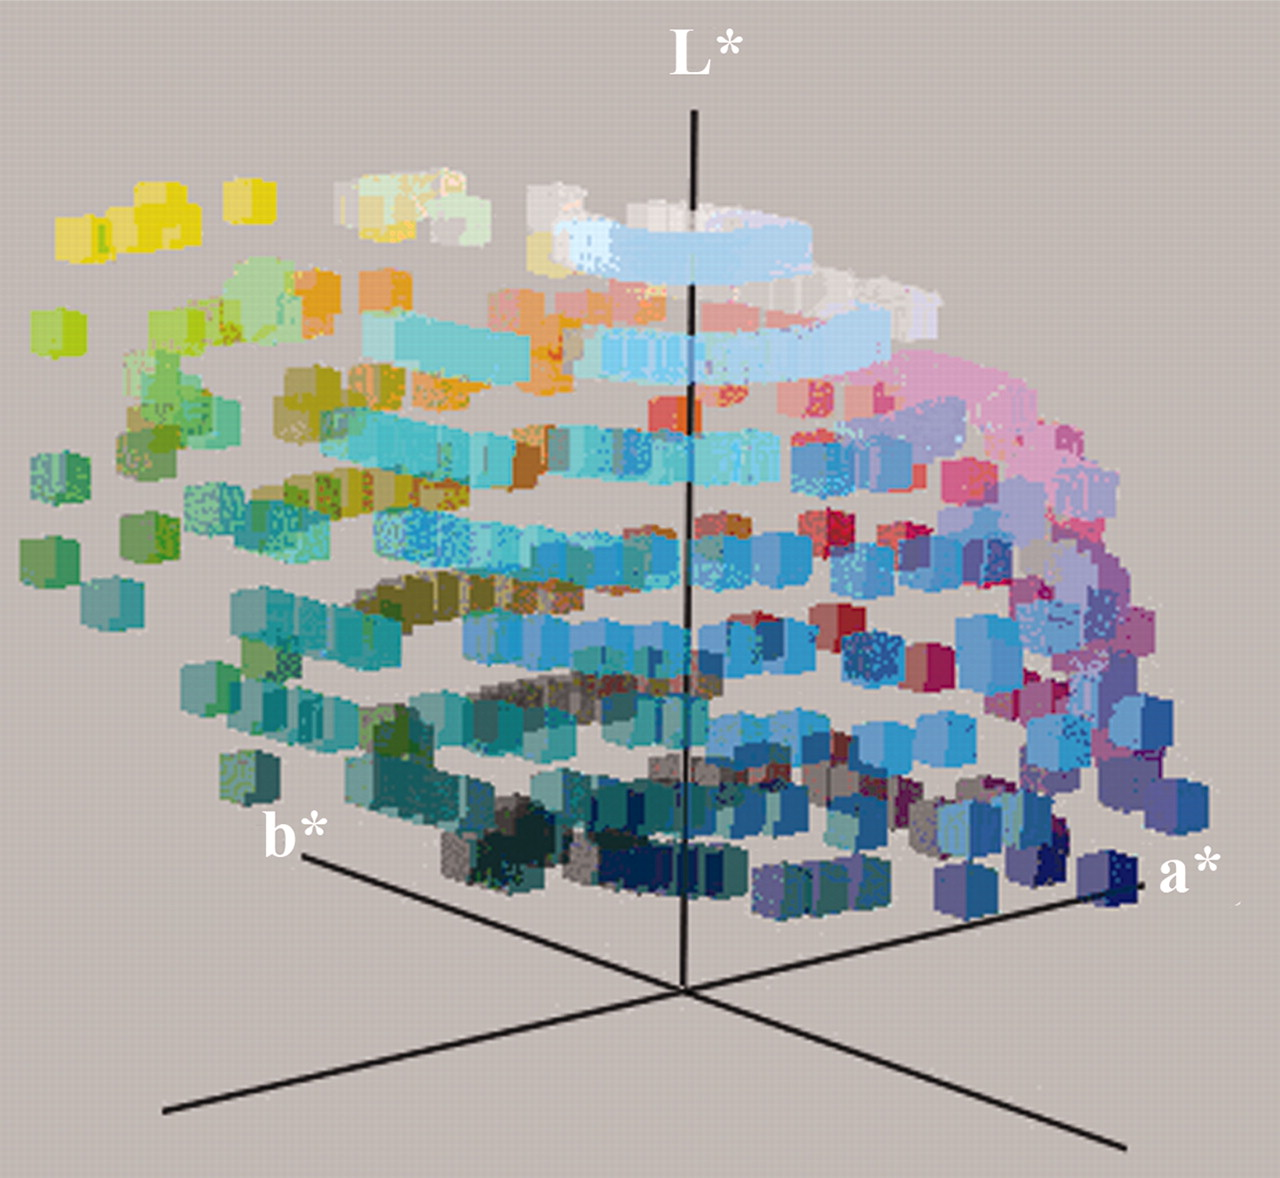
\includegraphics[width=\linewidth]{images/Cielab-space.jpeg}
\decoRule
\caption[Munsell Chips in Cielab Color Space.]{Munsell Chips in Cielab Color Space: 330 Musell color chips projected into Cielab color space. The irregular arrangement of the color chips is most prominent in the yellow region. \textcite{regierColor2007} used this irregularities and principles of categorization to explain the location and shape of color categories.
Taken from \textcite{regierColor2007}.}
\label{fig:Cielab_space}
\end{figure}

Subsequent theoretical work provided an alternative interpretation of the WCS findings. According to \textcite{regierColor2007}, the results of the WCS can be explained from two principles: a) a universally shared visual system, and b) an ``efficient'' organization of the lexicon. These universalist claims were pushed forward by an approach to predict color categories based on the mere irregularity of color space and basic assumptions of categorization. When converting the 330 color chips into the CIElab space, which constitutes a better psychophysical representation of the color space, the resulting locations of these color values do not yield a perfect symmetric shape (Fig. \ref{fig:Cielab_space}). 
A model using euclidean distances between color chips and rules of categorization to minimize similarity across categories and vice versa was able to predict naming patterns of real WCS languages. The model used a well formedness factor calculated as the sum of all distances of all chips of the same category and the distances of all chips that do not belong to the same category. When rotating the naming pattern along the L*axis, meaning to change the region of categories in the CIElab color space, the "Well-Formdness"-factor declined.
This was also true for languages that did not match the predictions of the model. Overall, these results support the hypothesis that color categories fit into optimal regions arranged by the universal peculiarities of color space \parencite{regierColor2007}.

% Change and add things
This idea was further developed by \textcite{zaslavskyEfficient2018}, proposing a unified formalization of “efficiency” using information theory. According to \textcite{zaslavskyEfficient2018}, efficient communication between speakers is characterized by an optimal trade-off between the complexity of the lexicon (as measured by the number of color terms) and the accuracy of communication. Therefore, languages with similar complexity have similar color maps because they provide similar optimal solutions to the problem of maximizing accuracy given a particular complexity.
The results of an iterated learning experiment performed by \textcite{xuCultural2013} are consistent with this communicative account. In the experiment, English-speaking participants were initially exposed to random assignments of color chips. The participants then generalized their responses to unseen chips after receiving some examples. The result of one participant was given to another participant, imitating cultural transmission in the real world. The systems of color terms produced by this process reproduced the structure of systems of color terms documented in the WCS.


Despite the impact of the World Color Survey, the data in the survey are limited to unwritten languages, mostly from small-scale societies and nonindustrial countries. Languages with many speakers, such as English, Spanish, French, and Portuguese, are missing from the survey. Part of the motivation for this omission was a concern that systems of color terms in industrial societies may have converged to similar structures as a result of contact through globalization. Data for these languages exist in the literature but are scattered in different papers with variations in methodology (for example, \textcite{forbesStructural1976, josserand:hal-03900005, lindseyColor2014, xuComparison2023}).


Several follow-up studies have further tested the findings of the WCS in a number of other languages and complementary paradigms. Most of these studies involved a small number of languages (e.g., German: \textcite{zollingerWhy1984}; Greek: \textcite{thierryUnconscious2009}; Turkish: \textcite{ozgenTurkish1998}). For example,\textcite{lindseyColor2014} asked participants to name colors in two different tasks. In the ``free elicitation task'', participants were asked to name colors freely using BCT, whereas, in the ``constrained naming task'', they had to use the eleven BCT elicited by \textcite{berlinBasic1969}.
Both groups showed fairly similar results with respect to the most frequently used color terms per color chip.

It is also well documented that some languages have greater diversity in terms of their shades of blue, in particular, Russian, Hebrew, and Italian \parencite{winawerRussian2007, CerquegliniHebrew, Paggetti2016ColorNI}. \textcite{winawerRussian2007} showed that Russian and English speakers differ not only in their color terminology, but also in the speed and accuracy of their discrimination of colors that fall into different color categories in one language and not the other.
% Several other languages also have a similar distinction between light and dark blue. For example,


% Color Term Evolution
Regarding Berlin and Kay's evolution hypothesis, follow-up studies declared to have found additional BCT for Russian \parencite{daviesBasic1994}, Greek \parencite{thierryUnconscious2009}, Turkish \parencite{ozgenTurkish1998} and German\parencite{zollingerWhy1984}. Another study by Lindsey and Brown proposed the stabilization of new color terms in English \parencite{lindseyColor2014}. This process of forming color categories is underpinned by a dual mechanism: it involves both the emergence between \parencite{levinsonYeli2000} and the partitioning \parencite{kayLinguistic1978} of preexisting color categories.
\parencite{lindseyColor2014}.
%They show, we can not be sure that previous datasets are not outdated by now.

Collecting new data could be specifically interesting to further deciphering these mechanisms of color term development especially for language where dataset already exist. Interestingly, several studies showed evidence for changes in the number of color terms within periods of just a few decades. For Japanese, for example, \textcite{kurikiModern2017} have reported that a large number of color categories have evolved significantly in less than fifty years. In another paper, \textcite{gibsonColor2017} documented changes in the number of color terms produced by Tsimane participants in the Bolivian Amazon and attributed these changes to industrialization due to the increased use of diversely colored artificial objects. In a large picture corpus investigation they discovered that objects are more likely to be colored in warm colors compared to the background. Subsequently, individuals exhibit increased precision and succinctness in naming warm color hues compared to their ability to articulate cold colors. Based on these observations, the researchers posited that the prevalent frequency of color usage acts as a catalyst, prompting the delineation and subsequent categorization of distinct chromatic nuances. In addition, they where able to show that Tsimane participants showed higher usage of color adjectives when describing artificial objects compared to natural objects. Thus, industrialization might drive the creation of new color categories simply by a greater use of diverse colored artificial objects.

\paragraph{\textbf{Color terms}}
The definition of BCT (BCT) is non trivial. The study of basic color term has long history (xxxxxxxx) but it was strongly promoted by aforementioned work by Berlin And Key \parencite{berlinBasic1969}.In this dissertation we operationally the definition to be commonly used in everyday life and not a compound word but a single word. Across the literature different explanations are given and different components are emphasized although this is a key factor to elicit comparable results \parencite{kayWorld2009 ,lindseyColor2014}. In fact, finding a definition that can be validly generalized across languages is a complex task. Some languages investigated during the WCS did not even have a word for color. In these cases experimenters were asked to use phrases like "How does it strike you eyes" \parencite{kayWorld2016}. In addition, the role and concept of compound words vary strongly across languages and make this definition less explicit. 
%In the case of Vietnamese it is not conclusively evident whether parts of a single word can be seperated by an "-" or if this already indicated that it is a compound word.


Another issue in the literature is the relationship between color terms and color categories. Often these two concepts are used interchangeably or mixed. However, this may poses problems, particularly when inferences are made from color terms and their use on color categories. \textcite{lindsey2009World} for example applied a k-means clustering algorithm on each individual naming pattern to identify a reasonable distribution of color categories independent of the actual term assigned. These categories are then named by the most common color term for this category. Even if they justify the level of this threshold the value remains arbitrary and distinct terms might be unified in single color categories. Therefore in the domain of color terms, clustering terms together is a strong unstable assumption. To avoid this loss of information, I propose alternative approach in this dissertation that does not commit to one category for each color. 
% Confusion of Color Categories and Terms
% A weakness in the studies mentioned so far is the confusion of color terms and categories.
% For the sake of clustering synonyms into one category the authors used k-means clustering to detect categories.
% However, we understand that in the domain of color terms, clustering terms together is a strong unstable assumption.
% Where to put the threshold to distinguish between two clusters?
% Especially in this research investigating the influence of language on perception we should stick to the actual color terms.
% Therefore, we propose that each color term should be treated as an own category.
% Hence, we strongly depend our analysis on color terms instead of clustered categories.

